\chapter{Theory}
This package contains a few simple two-dimensional geometric objects. The geometric objects are defined by a sufficient amount of points.
\subsection{Points}
A point $\mathbf{p}$ in a two-dimensional space can be described by its Cartesian coordinates
\begin{align}
    \mathbf{p} = \begin{pmatrix} x \\ y \end{pmatrix}.
\end{align}
If two points $\mathbf{p}_1$ and $\mathbf{p}_2$ are defined, we can connect those points using the connection vector $c$, which can be calculated by s the individual entires of $p_1$ and $p_2$
\begin{align}
    d  = \mathbf{p}_1 - \mathbf{p}_2 = \begin{pmatrix} x_1 \\ y_1 \end{pmatrix} - \begin{pmatrix} x_2 \\ y_2 \end{pmatrix}
\end{align}

\begin{figure}[h]
    \centering
    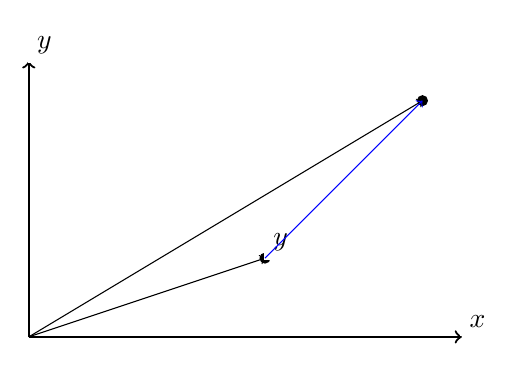
\begin{tikzpicture}
        %KOS
        \draw[->,thick,black] (0,0) -- (0,3.5);
        \draw (0.2,3.7) node [fill=white] {$y$};
        \draw[->,thick,black] (0,0) -- (5.5,0);
        \draw (5.7,0.2) node [fill=white] {$x$};

        \draw[->,thin,black] (0,0) -- (3,1);
        \fill[black] (3,1) circle (2pt);
        \draw (3.2,1.2) node [fill=white] {$y$};
        \draw[->,thin,black] (0,0) -- (5,3);
        \fill[black] (5,3) circle (2pt);

        \draw[->,thin,blue] (3,1) -- (5,3);
    \end{tikzpicture}
    \caption{some fig}
    \label{fig:lattice}
\end{figure}

\chapter{Software Design}
still tbd
